\section{\lare{}\label{lare}}
\subsection{Introduction}
\lare{}, lightweight \ajax{} replacement engine, is built on top of PJAX and successor of PJAXR.
\\
The idea of \lare{}, previous PJAXR, is to have the advantages of \ajax{} while trying to avoid it's disadvantages.
Introduced in Juli 2013, as an extended version of PJAX, it allows to replace multiple containers with a single request, instead of the limit to replace only one container.
Matching by the ID of an container it passed the duty to define which container should be replaced from the client-side to the server-side with setting the correct IDs.
Introducing the tags <lare-head>, besides a <lare-body> element, it reaches the ability to change meta tags, the page title and replace containers with only one request.
\\
This means it achieves the same UX improvements and reduced load times as classical \ajax{}.
On the other hand \singlePageApplication{}s using \lare{} are easily crawlable by the most used crawlers without additional efforts.
As successor of PJAXR it also uses the pushState function of the History interface to achieve full functionality of browsers incl. back- and forward buttons.
\lare{} is a generic solution for \singlePageApplication{}s and can be implemented in nearly every web application.

\subsection{Concept}

\begin{figure}[H]
\centering
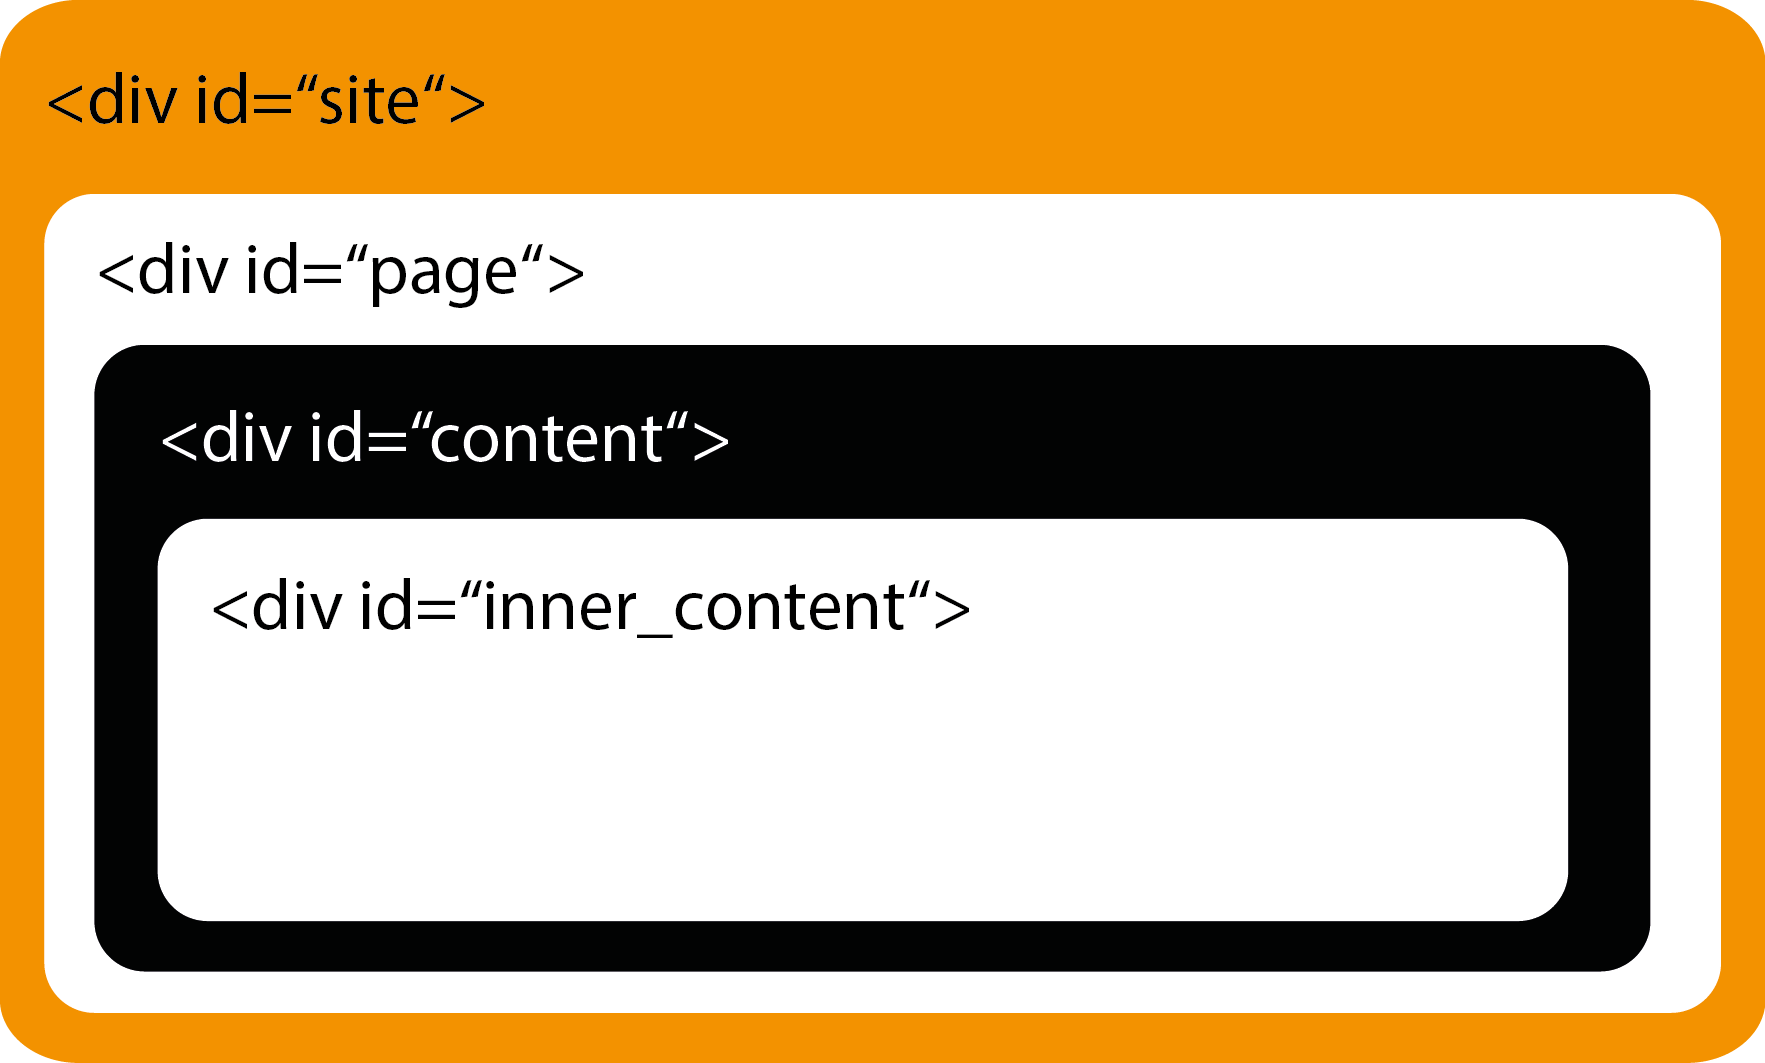
\includegraphics[width=13cm]{images/lare_html.png}
\caption[lare_html]{Basic HTML structure of a web application using \lare{}}
\label{fig:lare_html}
\end{figure}

Every \singlePageApplication{} which uses \lare{} has a hierachical namespace structure.
Typically the namespace consists of 4 levels: A site ID, a page ID, a content ID and an inner-content ID.
Every level in the hierarchy has it's counterpart on the website as shown in figure \ref{fig:lare_html}, a container with an ID telling which part of the namespace it belongs to.
\\
After the \lare{} frontend is initialized it hijacks events like clicks on links and enriches the request with the current website's namespace.
A \lare{} backend analyzes the namespace of the requested website and the one sent in the request.
For every hierarchy level it checks if both namespaces match.
If on one level the namespaces don't match the containers according to this level will be responded to the request.
An optimized web application only grabs the data necessary for those containers and render them afterwards.
The \lare{} frontend retrieves the response, replaces the containers at the website and updates the current namespace.

\begin{figure}[H]
\centering

\includegraphics[height=13cm]{images/lare.png}
\caption[lare_components]{Component and communication diagram of \lare{}}
\label{fig:lare_components}
\end{figure}

\noindent{}As shown in fig. \ref{fig:lare_components} the overall structure of \lare{} is similar to normal \ajax{} requests (compare fig. \ref{fig:ajax_components}).
The \ajax{} engine of \lare{} is \lareJS{}.
In addition to \ajax{}, \lare{} has a backend which helps to reduce server load and maps responses to the given namespace.
Optimally this analyzation is done as first action when retrieving a request by the web server.
Backend queries such database queries and such can then by left out if they are not necessary in the current namespace situation.


\subsection{Realization}
To load a page, the first request is a normal \httpRequest{} followed by a JavaScript script initializing the \lare{} frontend module.
Further requests to the same host are then initiated by this module.
The \http{} header of these requests is extended by the namespace of the current website.
The web server using a \lare{} backend compares the namespace of the requested resource and the namespace in the \http{} header.
It then decides which data is needed to be gathered and which template should be used to render those.
\\
The content delivered by the \lare{} backend enriched web server is interpreted by the frontend module and replaces the related containers.
This replacement is implemented using the ID attribute.
Other methods identifying corresponding containers like e.g. X-Path are not as generic in it's position on the page as the ID.
\\
Usage of the History API makes it then possible to update the content and change the URL like it would be made by normal requests.
This is possible with the use of the pushState method introduced in the History API.
Back- and forward-buttons and bookmarks in a browser will work like on a normal request using this function.
\\
Normal \httpRequest{}s and \lare{} requests request the same URL which makes it easy to crawl.
While on normal requests a full \webPage{} is responded \lare{} requests only get the changed containers as response.
Search engines and other crawlers are able to crawl every link it can find on a page and interpret it as normal \webPage{}s without any deficit.

\subsubsection{\lare{} frontend}

A \lare{} frontend has as mentioned before a few things to be implemented.
The first requirement is the ability to hijack page changes.
This can be implemented by e.g. replacing the default event listeners for anchor-tags.
A new event listener then has to implement an enrichment of the HTTP header by the namespace using the \enquote{HTTP-X-LARE} key.
On initial requests the current namespace should be served as an attribute at the <body> tag called data-lare-namespace.
\lare{} requests serve a new namespace as content of a tag <pjaxr-namespace>.
\\
As heart of \lare{} dynamic URL changes have to be implemented after getting the response.
This should be done by using the pushstate function.
\\
The biggest functionality of the \lare{} frontend is the replacement.
A response of a \lare{} request is divided into a <lare-head> tag, a <lare-body> tag and the <lare-namespace> tag.
Elements of the <lare-head> should be a new <title> tag and <meta> tags matching the new content. 
Additionally scripts or styles can be linked in this section when they are needed by the new content.
\\
The <lare-body> tag will contain the new content which should be replace old one.
Each container inside the <lare-body> will be searched by it's ID inside the current page and will then replace it's predecessor.

\subsubsection{\lare{} backend}

A \lare{} backend should first interpret the \enquote{HTTP-X-LARE} item in the HTTP header.
Every layer of the namespace should have it's own name.
As a default naming convention the layers should have the names \emph{site}, \emph{page}, \emph{content}, \emph{inner\_content} from start to the end.
Per layer a variable should save the matching state.
Those variables have to be accessible by views and controllers to give them the possibility to decide which backend requests should be made and which templates should be used.

\subsubsection{\lare{} templating}

To avoid a lot of overhead when using \lare{} a specific templating system is recommended.
\\
A default template for the first request could be like this:

\begin{minipage}[c]{0.95\linewidth}
\begin{lstlisting}[caption=Example Lare Base Template, label=example_lare_base_template]
<!Doctype html>
<html>
<head>
  <title></title>
  ...
</head>
<body data-lare-namespace="Lare.Namespace">
  <div id="site">
    ...
  </div>
</body>
</html>
\end{lstlisting}
\end{minipage}
\\
As shown above, it is a normal HTML5 template.
The only specific code you have to write when using \lare{} is the \emph{data-lare-namespace} attribute at the body tag.
\\
The \lare{} template has to be formed like this:

\begin{minipage}[c]{0.95\linewidth}
\begin{lstlisting}[caption=Example Lare Template, label=example_lare_template]
<lare-head>
  <title></title>
  ...
</lare-head>
<lare-body>
  <div id="site">
    ...
    <div id="page">
       ...
    </div>
    ...
  </div>
</lare-body>
<lare-namespace>Lare.Namespace</lare-namespace>
\end{lstlisting}
\end{minipage}
\\
The <lare-head> tag is the conterpart to the <head> tag, <lare-body> to <body>.
Instead of an attribute in the <lare-body> tag, the namespace will be delivered in the <lare-namespace> tag.
\\
For performance improvements it is intended to have a hierarchical structure as seen in fig. \ref{fig:lare_html}.
\\
When e.g. the first namespace matches, the <lare-body> could only deliver the page conatiner:

\begin{minipage}[c]{0.95\linewidth}
\begin{lstlisting}[caption=Example Lare Response, label=example_lare_response]
<lare-body>
  <div id="page">
    ...
  </div>
</lare-body>
<lare-namespace>Lare.AnotherNamespace</lare-namespace>
\end{lstlisting}
\end{minipage}



